\chapter{System Architecture and Design}
\label{ch:architecture}

\section{Architectural Overview}
The system is architected as an autonomous, closed-loop Software-Defined Network control platform designed to monitor kernel and physical datapaths, forecast incipient congestion episodes, compute constrained multipath bypasses, install safe OpenFlow 1.3 flow rules, and continuously verify post-reroute telemetry relief.

Figure~\ref{fig:arch_block_diagram} illustrates the end-to-end layered architecture of the platform.

\begin{figure}[H]
  \centering
  \begin{tcolorbox}[colback=white,colframe=sdnnavy,arc=3pt,title=\textbf{End-to-End System Layered Architecture}]
  \centering
  \small\sffamily
  \begin{tabular}{|c|}
    \hline
    \textbf{Layer 5: Visualization \& Human-in-the-Loop Operations}\\
    React 18 + TypeScript Console $\cdot$ Canvas Topologies $\cdot$ Strip Charts $\cdot$ LangGraph Agent Modal\\
    \hline
    $\Updownarrow$ \textit{WebSocket Telemetry Stream (2\,Hz) \& RESTful JWT API}\\
    \hline
    \textbf{Layer 4: Agentic Orchestration \& Decision Plane}\\
    LangGraph StateGraph Engine $\cdot$ LLM Cognitive Risk Assessment $\cdot$ OpenRouter API / Deterministic Fallback\\
    \hline
    $\Updownarrow$ \textit{Internal Python API \& Tool Execution Bus}\\
    \hline
    \textbf{Layer 3: Machine Learning \& Telemetry Analytics}\\
    Online Rolling Feature Pipeline $\cdot$ Random Forest Classifier $\cdot$ Calibrated Hazard Probability ($p$)\\
    \hline
    $\Updownarrow$ \textit{Port Counter Deltas \& Historical Sliding Windows}\\
    \hline
    \textbf{Layer 2: SDN Control Plane (Ryu Framework)}\\
    OpenFlow 1.3 Controller $\cdot$ Topology Discovery (LLDP) $\cdot$ Path Computation Engine $\cdot$ MBB Flow Dispatcher\\
    \hline
    $\Updownarrow$ \textit{OpenFlow 1.3 Southbound Channel (\texttt{OFPT\_PORT\_STATS}, \texttt{OFPFC\_ADD}, \texttt{OFPFC\_MODIFY})}\\
    \hline
    \textbf{Layer 1: Emulated Data Plane (Mininet + Open vSwitch + Linux TC)}\\
    Open vSwitch Software Switches $\cdot$ Virtual Ethernet Links (\texttt{veth}) $\cdot$ Netem Queue Buffers (100 pkts)\\
    \hline
  \end{tabular}
  \end{tcolorbox}
  \caption{Layered architecture of the autonomous closed-loop SDN optimization platform.}
  \label{fig:arch_block_diagram}
\end{figure}

\section{The Closed-Loop Control Cycle}
The heartbeat of the platform is the formal closed-loop control cycle, structured into five contiguous operational stages:

\begin{equation}
  \mathcal{C} = \left\langle \text{Observe}, \text{Predict}, \text{Decide}, \text{Reroute}, \text{Verify} \right\rangle
\end{equation}

\subsection{Stage 1: Observe (Telemetry Ingestion)}
The controller maintains an asynchronous polling task executing at a regular interval $T_{\text{poll}} = 2.0$\,seconds. For every active switch datapath identifier (DPID) and physical port $p$, the controller constructs and transmits an OpenFlow multipart port-statistics request:
\begin{lstlisting}[language=Python,caption={OpenFlow 1.3 port statistics request dispatch.}]
req = parser.OFPPortStatsRequest(datapath, 0, ofproto.OFPP_ANY)
datapath.send_msg(req)
\end{lstlisting}

Upon receiving the corresponding \texttt{OFPPortStatsReply}, the controller extracts cumulative byte counters $B_{\text{tx}}(t), B_{\text{rx}}(t)$ and packet counters $P_{\text{tx}}(t), P_{\text{rx}}(t), P_{\text{drop}}(t)$. Instantaneous link rate and utilization are computed against physical interface capacity $C$:
\begin{align}
  R_{\text{tx}}(t) &= \frac{(B_{\text{tx}}(t) - B_{\text{tx}}(t - \Delta t)) \times 8}{\Delta t \times 10^6} \quad [\text{Mbps}]\\
  U(t) &= \frac{R_{\text{tx}}(t)}{C} \times 100 \quad [\%]
\end{align}

\subsection{Stage 2: Predict (Incipient Hazard Inference)}
Instantaneous metrics are pushed into a fixed-size trailing sliding window $\mathcal{W}$ containing the most recent $N=12$ samples ($\sim 24$ seconds of continuous network history). The feature engineering pipeline computes rolling descriptive statistics:
\begin{equation}
  \mathbf{x}_t = \left[ \mu_U, \sigma_U, \text{slope}_U, \mu_{R}, \sigma_{R}, \text{slope}_{R}, \mu_{P}, \sigma_{P}, \text{drop\_ratio} \right]
\end{equation}
The vector $\mathbf{x}_t$ is passed to the trained Random Forest classifier $\mathcal{M}_{\text{RF}}$:
\begin{equation}
  p_t = P(\text{Congestion in } [t + 2\text{s}, t + 12\text{s}] \mid \mathbf{x}_t) = \mathcal{M}_{\text{RF}}(\mathbf{x}_t)
\end{equation}
If $p_t \ge \tau$ (calibrated decision boundary $\tau = 0.50$), the link is flagged as \textit{imminently hazardous}.

\subsection{Stage 3: Decide (Constrained Multi-Path Synthesis)}
Rather than allowing a machine learning model to directly emit raw OpenFlow rules (which carries severe hallucination and safety risks), the platform uses the predicted hazard probability $p_t$ as a dynamic penalty weight in a provably-safe path optimization cost function:

\begin{equation}
  \text{Cost}(e) = \alpha \cdot \frac{D(e)}{D_{\text{max}}} + \beta \cdot \frac{U(e)}{100} + \gamma \cdot p_t(e)
\end{equation}
where $D(e)$ is physical propagation delay, $U(e)$ is current utilization, $p_t(e)$ is the ML hazard probability, and $\alpha, \beta, \gamma$ are tuning weights (default: $\alpha=0.2, \beta=0.3, \gamma=0.5$). 

Using this dynamic cost graph $\mathcal{G}(V, E, \text{Cost})$, the decision engine executes Dijkstra's shortest path algorithm to identify the optimal primary path $P^*$ and an edge-disjoint alternate bypass path $P_{\text{detour}}$.

\subsection{Stage 4: Reroute (Make-Before-Break Flow Installation)}
When $P_{\text{detour}}$ is selected, the controller must install forwarding rules across all transit switches on the detour route. To guarantee that no in-flight packets are dropped during the transition, the platform enforces \textbf{Make-Before-Break (MBB)} installation semantics, described formally in Section~\ref{sec:mbb}.

\subsection{Stage 5: Verify (Closed-Loop Telemetry Affirmation)}
Following flow-mod dispatch, the controller does not assume the remediation was successful. Instead, the verify engine monitors subsequent telemetry samples over an observation window $T_{\text{verify}} = 4.0$\,seconds. The action is certified as \texttt{PASS} if and only if:
\begin{equation}
  U_{\text{bottleneck}}(t + T_{\text{verify}}) < 0.80 \quad \text{AND} \quad \text{Loss}(\%) \le 0.05
\end{equation}
If the verification condition fails, the controller escalates to secondary path selection or rate-shaping throttling.

\section{Network Topology Modeling}
To evaluate closed-loop control across diverse network environments, the platform defines a topology catalog comprising 10 distinct network architectures:

\begin{enumerate}
  \item \textbf{Double Diamond Multi-Path Fabric}: A canonical 4-switch, 4-host SDN testbed featuring two symmetric parallel multipath corridors between source switch $s_1$ and destination switch $s_4$: upper corridor $s_1 \leftrightarrow s_2 \leftrightarrow s_4$ and lower corridor $s_1 \leftrightarrow s_3 \leftrightarrow s_4$. Bottleneck links are configured with 10\,Mbps bandwidth and 100-packet buffer limits.
  \item \textbf{Internet2 Abilene WAN Backbone}: An 11-node, 14-link national wide-area transit network spanning continental United States Points of Presence (Seattle, Sunnyvale/SFO, Los Angeles/LAX, Denver/DEN, Dallas/DFW, Chicago/ORD, Atlanta/ATL, Indianapolis/IND, Washington D.C./WDC, New York/NYC).
  \item \textbf{Datacenter Fat-Tree ($k=4$)}: A hierarchical 3-tier fabric with 4 core switches, 8 aggregation switches, 8 edge switches, and 16 hosts.
  \item \textbf{Spine-Leaf Fabric}: A 2-spine, 4-leaf modern datacenter architecture.
  \item \textbf{Linear Chain (5 Switches)}: A serialized pipeline topology testing cascading queue delay.
  \item \textbf{Ring Fabric (6 Switches)}: A cyclic loop topology testing spanning-tree loop avoidance and bidirectional failover.
  \item \textbf{Grid Mesh ($3 \times 3$)}: A 9-switch grid testing dense multi-hop alternate route selection.
  \item \textbf{Clos Multi-Stage Fabric}: A 3-stage non-blocking switching network.
  \item \textbf{Full Mesh Core (5 Switches)}: A fully connected mesh with $\binom{5}{2} = 10$ core links.
  \item \textbf{Hub-and-Spoke Enterprise Fabric}: A central aggregation core connecting 6 remote branch offices.
\end{enumerate}

\begin{figure}[H]
  \centering
  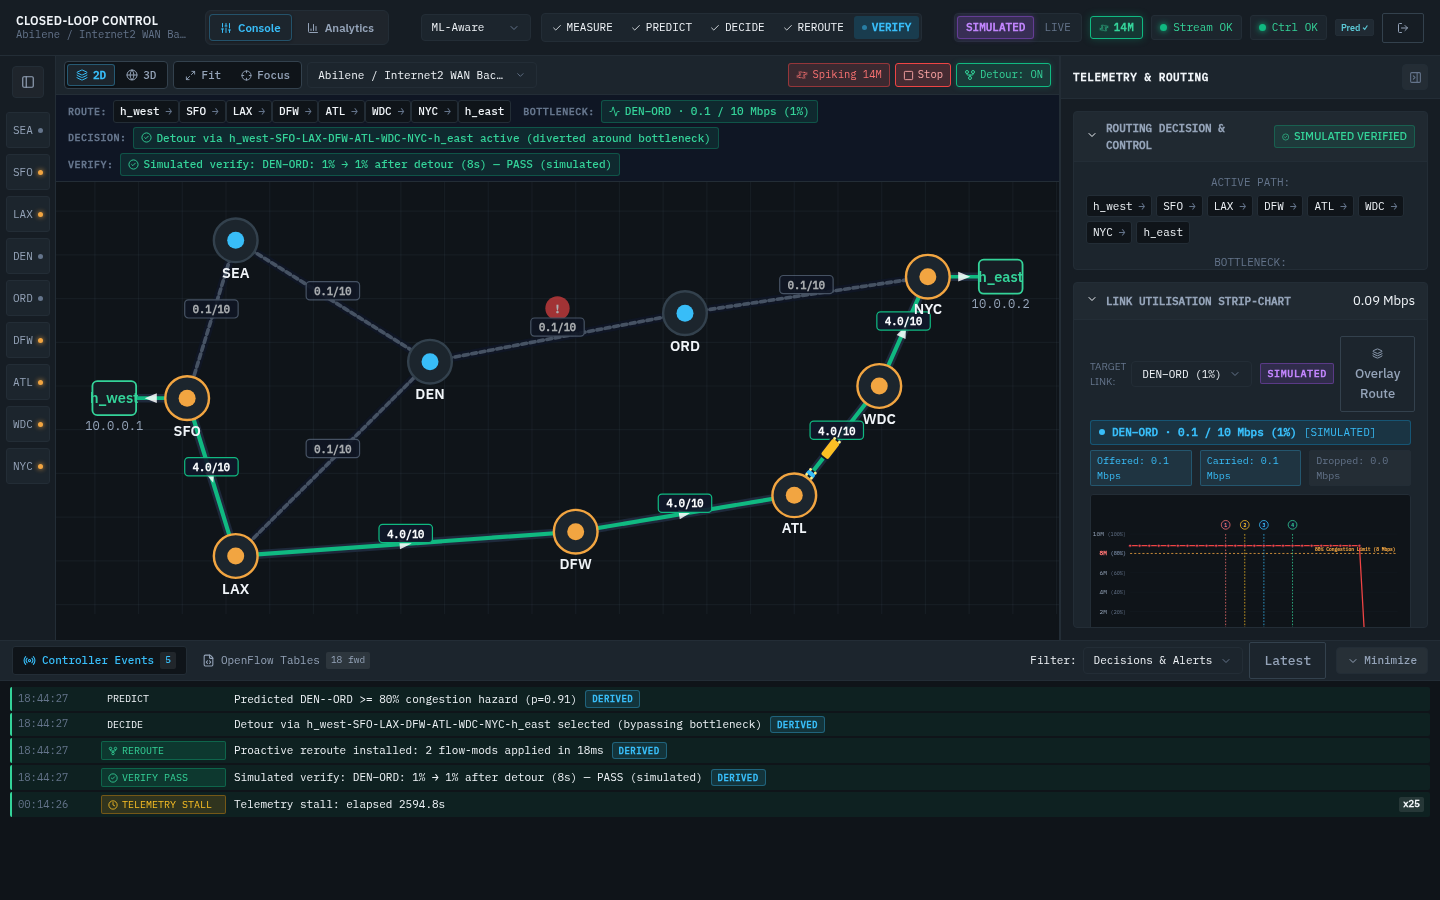
\includegraphics[width=0.88\textwidth]{results/snapshots_ui_fixes/fixed_abilene_detour_pass.png}
  \caption{Internet2 Abilene 11-node WAN topology rendered live in the interactive visualization console following Make-Before-Break detour installation.}
  \label{fig:abilene_console_view}
\end{figure}

\section{Make-Before-Break (MBB) Flow Installation Semantics}
\label{sec:mbb}
A frequent cause of packet loss during network rerouting is \textit{transient black-holing}. If an ingress switch diverts packets onto a new path before downstream intermediate switches have installed their matching forwarding entries, packets arriving at intermediate switches trigger table-miss events, causing packet drops or flooding the controller with unexpected \texttt{OFPT\_PACKET\_IN} messages.

\begin{tcolorbox}[colback=codebg,colframe=sdnnavy!80,arc=3pt,title=\textbf{Algorithm 1: Make-Before-Break (MBB) Flow-Mod Installation Protocol}]
\small\sffamily
\textbf{Input}: Detour path $P = \langle s_{\text{in}}, s_1, s_2, \dots, s_k, s_{\text{out}} \rangle$, Match criteria $M$, Priority $p_{\text{high}}$\\
\textbf{Output}: Traffic rerouted onto $P$ with zero transient packet drops or loops\\[0.2cm]
\textbf{Phase 1: Downstream Forward Path Pre-Programming}
\begin{enumerate}[leftmargin=1.5em,noitemsep]
  \item \textbf{for} $i = k$ \textbf{downto} $1$ \textbf{do}:
  \item \quad $\text{dp} \gets \text{GetDatapath}(s_i)$
  \item \quad $\text{out\_port} \gets \text{GetEgressPort}(s_i \to s_{i+1})$
  \item \quad $\text{rule} \gets \text{ConstructFlowMod}(\text{Match}=M, \text{Action}=\text{Output}(\text{out\_port}), \text{Priority}=p_{\text{high}})$
  \item \quad $\text{dp}.\text{send\_msg}(\text{rule})$
  \item \quad $\text{BarrierRequest}(\text{dp})$ \quad \textit{// Enforce hardware TCAM commit before upstream shift}
\end{enumerate}
\textbf{Phase 2: Ingress Switch Flow Redirection}
\begin{enumerate}[leftmargin=1.5em,noitemsep,resume]
  \item $\text{dp}_{\text{in}} \gets \text{GetDatapath}(s_{\text{in}})$
  \item $\text{out\_port}_{\text{new}} \gets \text{GetEgressPort}(s_{\text{in}} \to s_1)$
  \item $\text{ingress\_rule} \gets \text{ConstructFlowMod}(\text{Match}=M, \text{Action}=\text{Output}(\text{out\_port}_{\text{new}}), \text{Priority}=p_{\text{high}})$
  \item $\text{dp}_{\text{in}}.\text{send\_msg}(\text{ingress\_rule})$
  \item $\text{BarrierRequest}(\text{dp}_{\text{in}})$
\end{enumerate}
\textbf{Phase 3: Drain and Safe Rule Teardown}
\begin{enumerate}[leftmargin=1.5em,noitemsep,resume]
  \item $\text{Sleep}(\Delta t_{\text{drain}})$ \quad \textit{// Allow in-flight packets on old path to exit queues}
  \item $\text{RemoveDeprecatedRules}(\text{OldPath}, M)$
\end{enumerate}
\end{tcolorbox}

As formalized in Algorithm~\ref{alg:mbb}, rules are installed in strict reverse topological order from the destination-adjacent switch back to the ingress switch, accompanied by OpenFlow barrier synchronization requests (\texttt{OFPT\_BARRIER\_REQUEST}). This guarantees that every downstream forwarding entry is committed in switch TCAM before the ingress switch redirects the initial packet of the flow.
